\chapter{Frontend Design}

\section{Introduction}
\lettrine[lines=2]{I}\\n this chapter, we will summarise all the previous research, with a particular focus on users, book format reading experience, sharing, communication and other functions in detail. 
At the same time, we will filter the common E-book formats available on the market from a technical perspective, expecting to find a suitable format among them.

\section{Research summary}

The structure of the book resources shown as Fig~\ref{fig30} is supported by most of the current platforms. 

\begin{figure}[htbp]
  \centerline{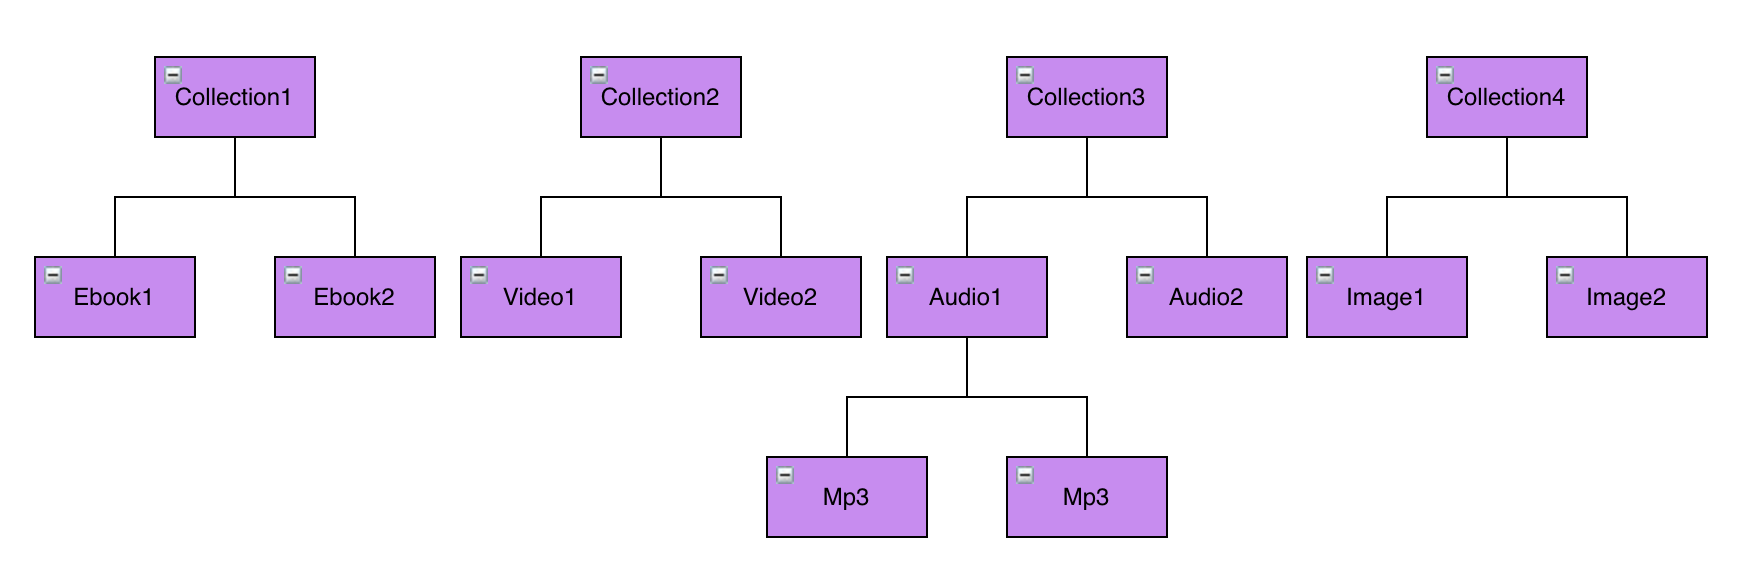
\includegraphics[width=500pt]{images/collections.png}}
  \caption{Collections}
  \label{fig30}
\end{figure}

Commonly supported data formats are E-books, audio, video and pictures. 
They are all grouped together by subject, similar to how a library book index is managed. 
Because the audio is often in the form of a playlist, it is a little deeper in the hierarchy. 

User sharing and connection is a weakness of these platforms.
This is because the fact that platforms are often seen as purely online libraries.
It is common that a platforms do not take into account the online user community.

\section{Demo}

In this initial demo, our main considerations are compatibility and usability.

\subsection{compatibility}

Because the user range is 13 to 18 years old and there is a possibility of future expansion to other user ranges, compatibility is the first thing. 
This is because good compatibility across multiple devices will minimise the cost of future development for the habits of different age groups.
They can use this platform on multiple devices.

As same as other common platforms, we can take HTML5 responsive development to get an interface that is compatible with both pc and mobile devices.
So that only one development is needed to get a consistent user experience on PC, mobile, ipad and other devices at the same time.

\subsection{usability}

Usability is mainly concerned with the different experiences with different file formats.
It is also known as the reader experience. 

\subsubsection{Books}

A reader in book format is shown in the left of Fig~\ref{fig31}.
The most important elements are page turning, sharing and commenting. 
Turning pages allows a book to be partly free and partly paid for or partly open to visitors in the future. 
Sharing and commenting is a very important place to keep people of the tribe connected. 

\begin{figure}[htbp]
  \centerline{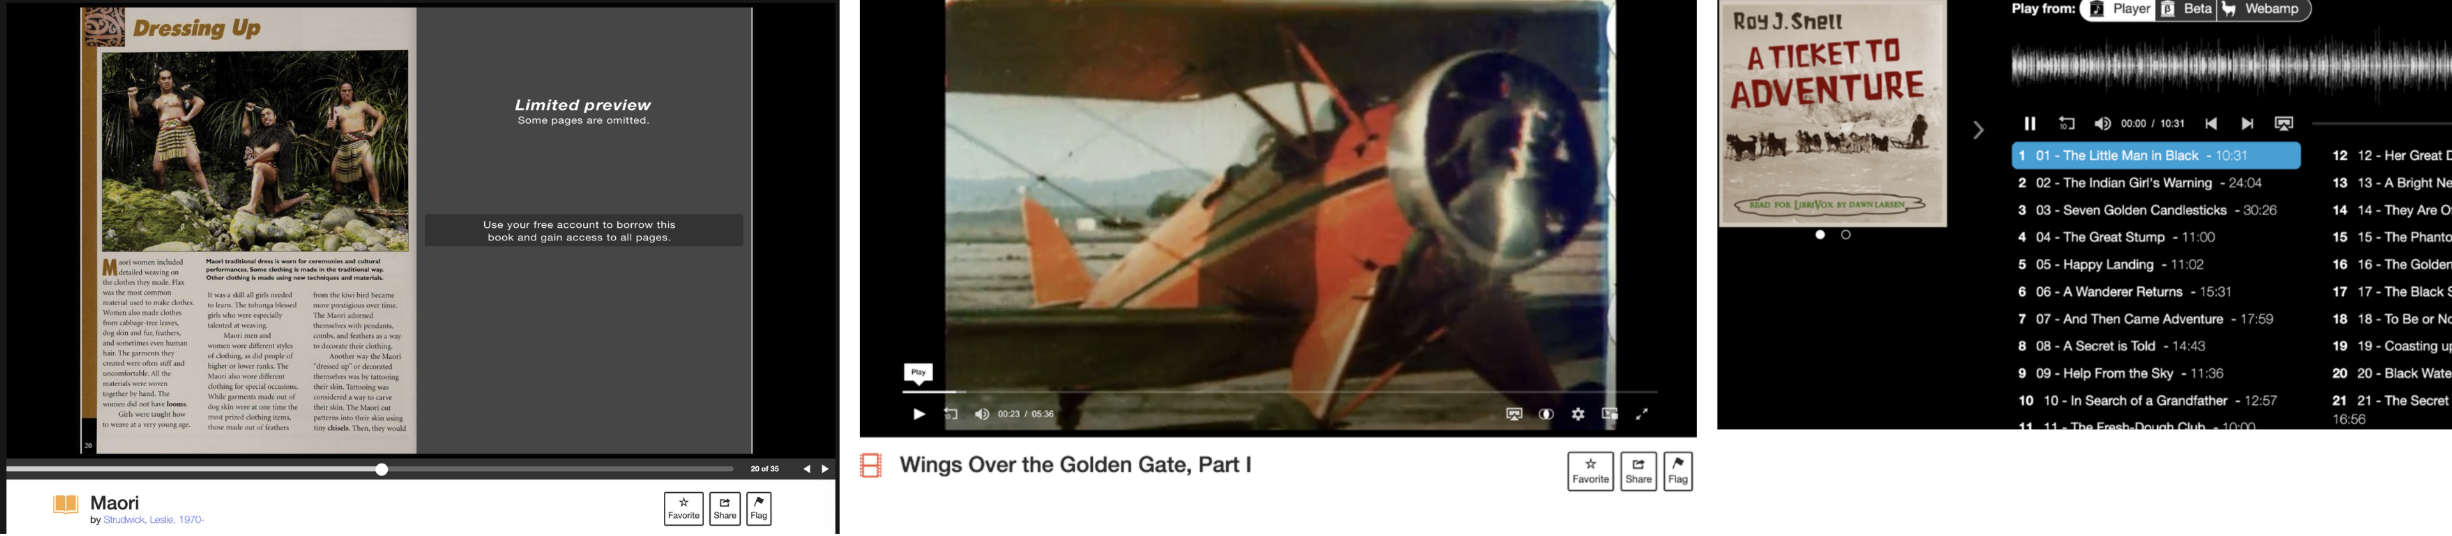
\includegraphics[width=500pt]{images/Book.png}}
  \caption{Books, Videos, Audios Readers}
  \label{fig31}
\end{figure}

\subsubsection{Videos}

The reader for videos is shown in the middle of Fig~\ref{fig31}. 
It needs to be a very versatile video player. 
Unlike the last one, its key features need to include subtitles, volume, progress bars and so on.

\subsubsection{Audios} 

The reader for audios is shown in the right of Fig~\ref{fig31}. 
It needs to work as well as some mp3 online players. 
Its important features need to include previous song, next song, jumbled play and possibly lyrics like subtitles too.

\subsubsection{Images}

The reader for images is similar as books. 
There may be a need for a previous next picture viewing mode.
And there may be a choice of resolutions to suit the speed of the network.

\section{E-book formats}
We have collected and collated a range of E-book data formats (Table \ref{fig32}) and selected the ones that suit this project.
They are only aggregated from a technical level so they are senseless to end users. 
In the actual project, there is also the possibility of adapting the final data format to suit the trade-off between network speed and resource quality.

On the other hand, if the current file formats fail to meet the requirements, it may be necessary to develop a proprietary format to achieve the optimal user experience.

\begin{table}[h]
  \centering
  \caption{Ebook formats}
  \begin{tabular}{|c|p{10cm}|}
  \hline
  \textbf{Ebook format} & \textbf{Description} \\
  \hline
  EPUB & A widely used open standard for ebooks that supports reflowable text, inline images, and DRM. EPUB files can be read on a variety of devices and platforms. \\
  \hline
  PDF & A popular format for ebooks that preserves the original formatting and layout of the document. PDF files can be viewed on a wide range of devices, but may not be optimized for smaller screens. \\
  \hline
  MOBI & A format developed by Amazon for use on their Kindle devices. MOBI files support advanced features such as reflowable text, adjustable fonts, and inline images. \\
  \hline
  Markdown & A lightweight markup language that is easy to write and read. Markdown files can be easily converted to a variety of formats including HTML, PDF, and EPUB. \\
  \hline
  HTML & A web-based format for ebooks that can be read in any modern web browser. HTML files can include advanced features such as multimedia content and interactive elements. \\
  \hline
  \end{tabular}
  \label{fig32}
  \end{table}
  

\section{Overall conclusion} 

This report involved extensive market research and analysis, leading to the development of a initial demo that meets the requirements. 
While we recognize that further communication and collaboration will be necessary to refine the final prototype.
We are confident that this project has the potential to provide the iwi with a powerful electronic platform for sharing and connections. 

This project holds significant importance for Waikatōhea iwi, because it aims to digitize the collection of books and create an electronic platform that can be accessed by iwi members and others. 
By sharing iwi's culture and history through this platform, we hope to strengthen iwi community and build connections with each other. 
This project is a step towards preserving the heritage and making it accessible to future generations.


